\documentclass[10pt]{article}
\usepackage[margin=0.5in]{geometry}
\usepackage{amsmath}
\usepackage{enumitem}
\usepackage{multicol}
\usepackage{tikz}
\usepackage{soul}

\newcommand{\ds}{\displaystyle}

\begin{document}
\newcounter{enumCount}
\pagestyle{empty}
\subsection*{Homework 3 - Math 140 \hfill Name: \underline{\hspace*{2in}}}


\noindent 
\textit{Simplify each expression.}
\begin{multicols}{3}
\begin{enumerate}
\setcounter{enumi}{\theenumCount}
\item $x^2 (5x^7)$.
\item $(4x^3)^2$.
\item $\dfrac{(2x)^3}{6 x^2}$.
\setcounter{enumCount}{\theenumi}
\end{enumerate}
\end{multicols}
\vfill

\noindent
\textit{Simplify and rewrite without negative exponents.}
\begin{multicols}{3}
\begin{enumerate}
\setcounter{enumi}{\theenumCount}
\item $\frac{1}{2} (x^{-3})$.
\item $\left(\dfrac{x^3}{2}\right)^{-3}$.
\item $\dfrac{8 \, x^{-5}}{6 \, x^{-3}}$.
\setcounter{enumCount}{\theenumi}
\end{enumerate}
\end{multicols}
\vfill

\noindent 
\textit{Rewrite using negative and/or fractional exponents, so there are no radical symbols.}
\begin{multicols}{3}
\begin{enumerate}
\setcounter{enumi}{\theenumCount}
\item $\dfrac{3}{\sqrt{x}}$.
\item $x \sqrt[4]{x}$.
\item $\dfrac{x}{\sqrt[3]{x}}$.
\setcounter{enumCount}{\theenumi}
\end{enumerate}
\end{multicols}
\vfill


\begin{multicols}{2}
\begin{enumerate}
\setcounter{enumi}{\theenumCount}
\item Has a slope of 5 and crosses the $x$-axis at $x=3$.
\item Passes through $(3,4)$ with slope of $-6$.
\setcounter{enumCount}{\theenumi}
\end{enumerate}
\end{multicols}
\vfill


\begin{enumerate}
\setcounter{enumi}{\theenumCount}
\item Find the slope and $y$-intercept of the line $4x + 6y = 24$.
\vfill


\item A clothing business finds there is a linear relationship between the number of shirts, $n$, it can
sell and the price, $p$, it can charge per shirt. In particular, historical data shows that 1000
shirts can be sold at a price of \$30, while 3000 shirts can be sold at a price of \$22 . Find a
linear equation in the form $p = mn + b$ that gives the price $p$ they can charge for $n$ shirts.\vfill

\item How many shirts would the business be able to sell if the price was \$20? 
\vfill


\newpage

\item  Suppose that the cost for a business to manufacture $x$ widgets is $C(x)$ dollars.  Explain in words what the following equation means:
$$C(5{,}000) = 6{,}000.$$
\vfill
\setcounter{enumCount}{\theenumi}
\end{enumerate}



\noindent
\textit{Suppose that $f(x) = \dfrac{1}{x+2}$ and $g(x) = 4x+3$.}
\begin{multicols}{2}
\begin{enumerate}
\setcounter{enumi}{\theenumCount}
\item Calculate $f(g(0))$.
\item Calculate $g(f(0))$.
\setcounter{enumCount}{\theenumi}
\end{enumerate}
\end{multicols}
\vfill

\noindent
\textit{The following graphs show two different functions $f(x)$ and $g(x)$.}

\begin{center}
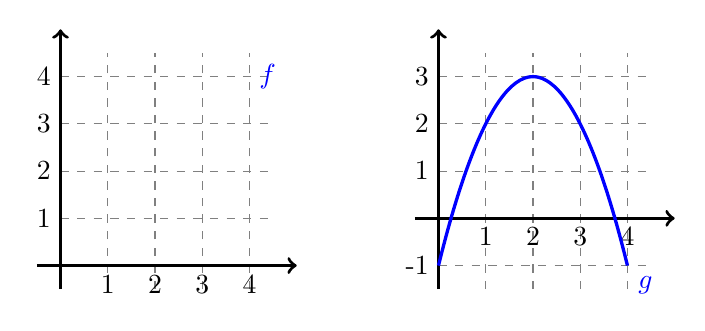
\begin{tikzpicture}[scale=0.6]
\draw[dashed, gray] (0,-0.5) grid (4.5,4.5);
\draw[very thick,->] (-0.5,0) -- (5,0);
\draw[very thick,->] (0,-0.5) -- (0,5);
\foreach \i in {1,...,4} {
  \draw (\i,0) node[below] {\i};
  \draw (0,\i) node[left] {\i};
}
\draw[very thick,color=blue] plot[domain=-0.5:4.1,samples=100] function {4/(5-x)};
\draw[color=blue] (4,4) node[right] {$f$};
\begin{scope}[xshift=8cm, yshift=1cm]
\draw[dashed, gray] (0,-1.5) grid (4.5,3.5);
\draw[very thick,->] (-0.5,0) -- (5,0);
\draw[very thick,->] (0,-1.5) -- (0,4);
\foreach \i in {1,...,4} {
  \draw (\i,0) node[below] {\i};
}
\foreach \i in {-1,1,2,3} {
  \draw (0,\i) node[left] {\i};
}
\draw[very thick, blue] (0,-1) parabola bend (2,3) (4,-1) node[below right] {$g$};
\end{scope}
\end{tikzpicture}
\end{center}
\textit{Use the graphs to evaluate the following.}
\begin{multicols}{3}
\begin{enumerate}
\setcounter{enumi}{\theenumCount}
\item $f(g(2))$
\item $g(f(1))$ 
\item $g(f(4))$ 
\setcounter{enumCount}{\theenumi}
\end{enumerate}
\end{multicols}
\vfill


\end{document}
